
\documentclass[12pt]{article}

\usepackage{amsmath}
\usepackage{amssymb}
\usepackage{epsfig}
\usepackage{epstopdf}
\usepackage{algorithm}
\usepackage{algpseudocode}
\usepackage{amsfonts}
\usepackage{mathtools}
\usepackage{upgreek}
\usepackage{tikz}
\usepackage{verbatim}

\usepackage{multirow}
\usepackage[T1]{fontenc}
\usepackage{beramono}
\usepackage{listings}
\usepackage{xcolor}
\definecolor{backcolour}{rgb}{0.95,0.95,0.92}

\lstdefinelanguage{Julia}%
{morekeywords={abstract,break,case,catch,const,continue,do,else,elseif,%
		end,export,false,for,function,immutable,import,importall,if,in,%
		macro,module,otherwise,quote,return,switch,true,try,type,typealias,%
		using,while},%
	sensitive=true,%
	morecomment=[l]\#,%
	morecomment=[n]{\#=}{=\#},%
	morestring=[s]{"}{"},%
	morestring=[m]{'}{'},%
}[keywords,comments,strings]%

\lstset{%
	language         = Julia,
	keywordstyle     = \bfseries\color{blue},
	stringstyle      = \color{magenta},
	commentstyle     = \color{gray},
	backgroundcolor= \color{backcolour}, 
	basicstyle=\footnotesize,
	showstringspaces = false,               
	numbers=left,                    
	numbersep=5pt,                 
	tabsize=4
}


\begin{document}

\title{CSCE 686 Homework 5 - SCP Design}
\author{Jon Knapp and Justin Fletcher}
\maketitle

\section{Talbi 1.5 [a]}
\textit{Show that it is easy to find a simple greedy heuristic that guarantees a 2-approximation factor for the minimum vertex covering problem.}
\linebreak

Given a graph, $G=(V, E)$, the vertex cover is a set of vertices such that every edge touches, or is incident to, at least one of them \cite{Lecture21}. An unweighted minimum vertex cover is, is the smallest possible set of vertices which covers all edges \cite{Dartmouth}, and is formally defined as
\begin{align*}
I\subseteq V(G) 
\end{align*} 
where,
\begin{equation*}
\min |I| \\
\end{equation*}
\begin{equation*}
\; s.t. \; E(G)\subseteq \bigcup_{u,v \in I}\{uv\}.
\end{equation*}
If the vertices are weighted, and the minimum-weight vertex cover is desired, then the minimization constraint becomes 
\begin{equation*}
\min \sum_{v\in I} w(v).
\end{equation*}
Without a heuristic, this problem is NP-Hard. In order to approximate the solution, we introduce a matching in $G$. A matching is a set of edges such that no two edges are incident to a common vertex \cite{Suhendry}. A vertex is thus matched, or saturated, if an edge in the matching is incident to that vertex. A maximal matching $M$ is obtained when no further edges can be added to $M$ without violating the matching constraint.

The maximal matching is related to the vertex cover \cite{Suhendry}, in that a valid vertex cover is also the set of all endpoints in any maximal matching $M$. To illustrate this concept, two graphs are shown in Figure  \ref{fig:maximalmatchings}, where the set of endpoints for any maximal matching, depicted as bold lines, also forms a valid vertex cover.


\begin{figure} \label{fig:maximalmatchings}
	
	
		
		\centering
		\centerline{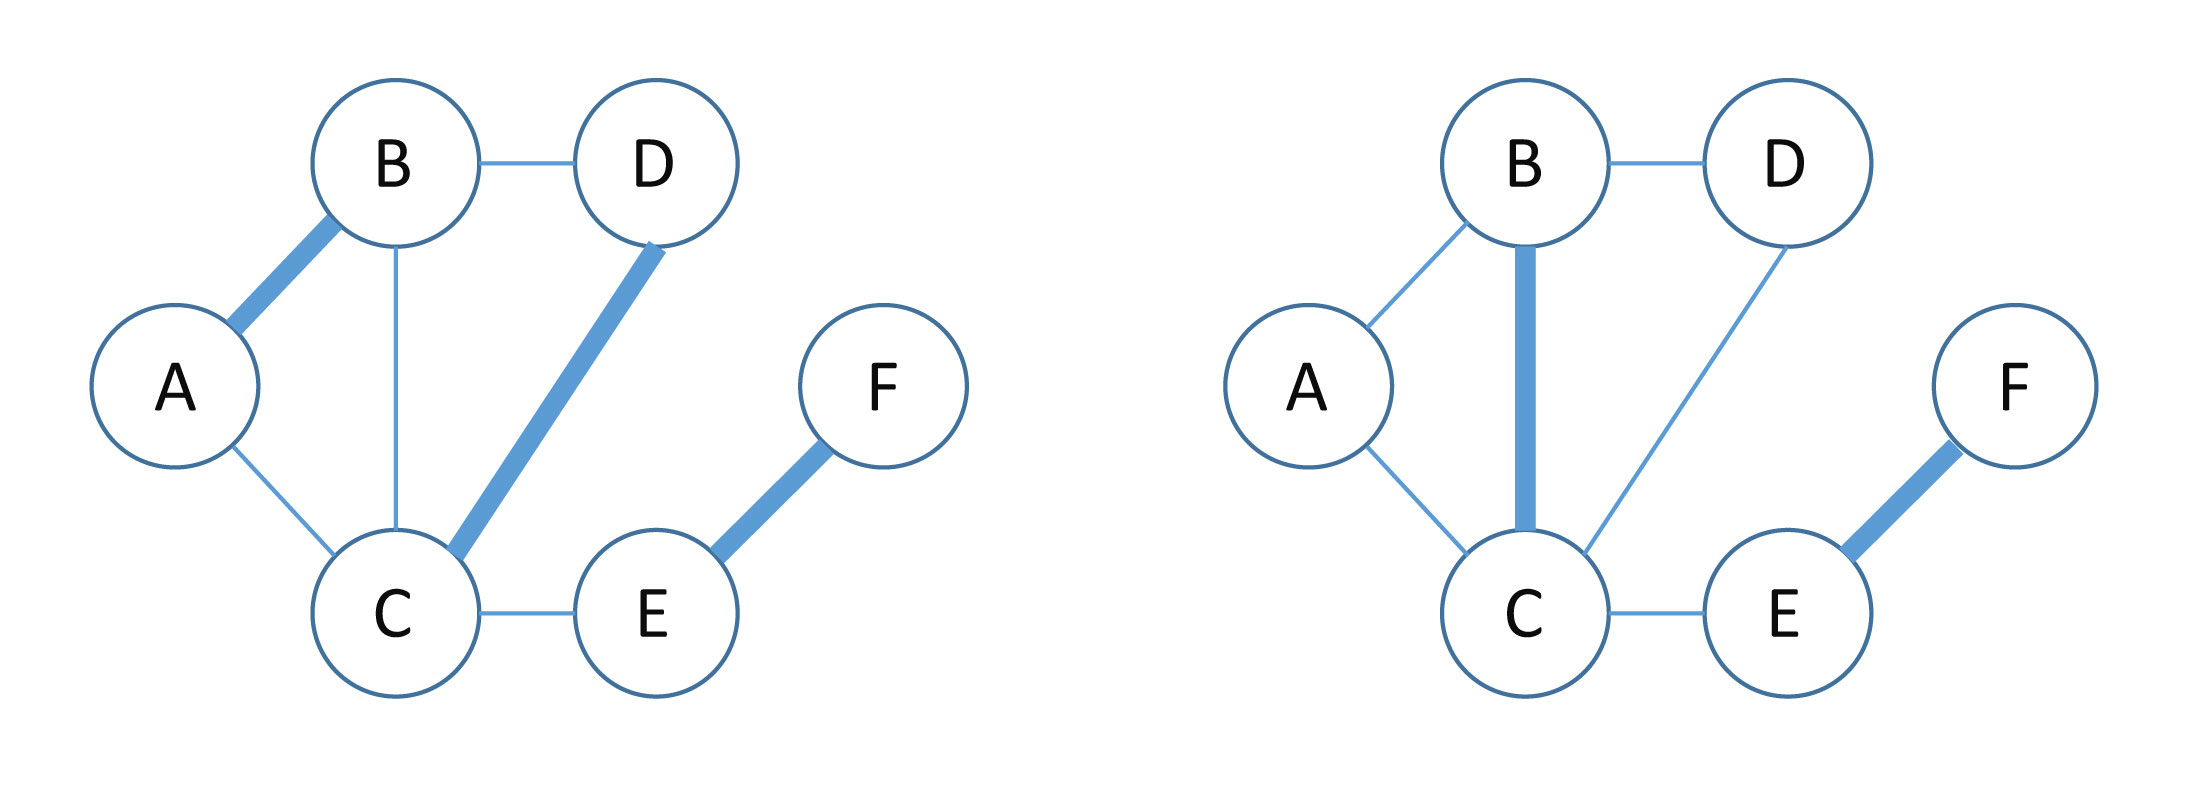
\includegraphics[width = 5in]{FigureA.jpg}}
		%  \vspace{2.0cm}
	\hfill
	
	%\vspace{-0.5cm}
	\caption{This figure displays two examples of maximal matching, shown as bold edges.}
	
	
\end{figure}

If we assume that some vertex set $I \subseteq V(G)$ is the minimum vertex cover for $G$, then we also know that $|I| \geq |M|$, where $M$ is any maximal matching. $I$ must contain at least one of vertices to which every edge in $M$ is incident, in order to cover all edges in $G$. Since no more edges can be added to a maximal matching, all remaining edges are adjacent to at least one edge in $M$. We can cover the entire graph by choosing the endpoint vertices to all edges in $M$.

We define an algorithm, $GetM$, to produce $M$, which is included as Algorithm \ref{alg:get2Approx} in this work. The algorithm produces a maximal matching. All pairs of vertices that are added into $C$ are unique, and thus eliminating any edges that share a vertex. The algorithm only terminates when there are no uncovered edges. Using this relationship, we conclude that the following:


\begin{algorithm}[ht!]
	\caption{This algorithm describes 2-approximation heuristic. \textit{Inputs:} $E$, a set of edges.
		\textit{Outputs:} Set of vertices $C$.} 
	\begin{algorithmic}[1]
		
		
		\Procedure{get2Approx}{$E$}
		\State $C \gets \phi$ 
		%\State $E \gets$ set of edges
		\While{($u, v$) not covered, and $u \neq v$} \Comment{Iterate over every potential edge }
		\State Add $u$ to $C$.
		\State Add $v$ to $C$.
		\EndWhile
		\EndProcedure
		
	\end{algorithmic}	
	\label{alg:get2Approx}
\end{algorithm}



\begin{align*}
|I|  \geq |M| = GetM(G) / 2
\end{align*}
The vertex cover is size $2M$. The previous relationship can be written as:

\begin{align*}
GetM(G) \leq 2 |I|
\end{align*}

The heuristic that we presented uses the relationship between matching sets and the set covering problem. By finding a maximal matching, we can $2$-approximate the minimum vertex cover problem with $O(m)$ complexity.



\section{Talbi 1.11 [a]}

\textit{Define one or more greedy algorithms for the CVRP problem. Give some examples of constraints or more general models encountered in practice.}

The Capacitated Vehicle Routing Problem (CVRP) is defined by a Graph $G = (V, A)$. The nodes represent "customers" and $A$ defines costs, denoted as $c_{ij}$, associated with each edge. Additionally, a central "depot" node is defined, as well as a capacity $Q$ for each "vehicle," associated with each "route" [ref MCT1]. A depot can only have $H$ number of routes. Customers have an associated demand, $d_i$, which defines the quantity that will be used to calculate the total capacity of a route. This problem finds routes for a fleet of vehicles so that every customer is covered and no vehicle exceeds its capacity.

A well-known algorithm for solving the CVRP is the Clarke and Wright Savings (CWS) algorithm, developed in 1964 [2]. It is a greedy, heuristic driven algorithm that does not guarantee an optimal solution, although it will often provide a good solution [3]. This method is initialized by assuming that each customer (non-depot node), is visited by its own vehicle. If the graph consists of the depot node A, and two customers $i$ and $j$, the cost $D1$, is calculated using the formula

\begin{align*}
D_1 = c_{Ai} + c_{iA} + c_{Aj} + c_{jA}
\end{align*}

The algorithm combines routes to obtain a new route by assigning two customers to be served by the same vehicle, assuming the vehicle's capacity Q has not been exceeded. The new cost is

\begin{align*}
D_2 = c_{Ai} + c_{ij} + c_jA
\end{align*}

A total cost savings, $S_{ij}$, is calculated:

\begin{align*}
S_{ij} = D_1 – D_2 = c_{iA} + c_{Aj} – c_{ij}
\end{align*}

This saving is used to determine if the points $i$ and $j$ should be on the same route. Large values of S indicate that the route is advantageous. 
The algorithm starts by calculating the savings for all pairs of customers and putting them in a sequence $R$. This sequence is then sorted in descending order of the savings. When considering a pair of points $i$ and $j$ whose capacity is less then $Q$ for a particular route, they are added to the route such that $i$ is visited and then $j$, but only if this can be done without disrupting the direct connection between two nodes. In the parallel version of this algorithm, only one pass is required through $R$, and routes are built simultaneously [3].

Not only does this algorithm not guarantee an optimal solution, it cannot guarantee that the number of routes will be exactly $H$. A particular execution of the algorithm may find some $H^\prime$ greater then $H$. However, using the savings heuristic it can produce a solution that is usually close to optimal [4].

There are a wide variety of solutions to the CVRP in the literature that use Monte-Carlo techniques to improve the search. One such algorithm, described in [2], uses a random sampling to acquire a solution.

In practice, there are many additional constraints for CVRP problems. One such domain is the oil and gas industry [4]. For particular delivery vehicles, the presence of flow meters can be used to satisfy the demands of multiple customers. Additionally, after certain operations, the delivery vehicles may require cleaning, which must be factored into the route plan. Although not specifically mentioned in the source, the presence of refueling stations would constrain the routes further.

Another domain that can constrain VRP problems is retail. For any particular product supplier, the cost of delivering goods to stores is a significant investment. This cost can be reduced with CVRP algorithms. From personal experience in the industry, we use the floral industry as a hypothetical example. The constraints for this application include not combining certain products (some flowers and plants cannot be shipped together), always sending certain drivers to a particular customer (customer loyalty), delivering highly perishable goods first, or long lived items last. Additional considerations include how profitable a particular customer is and the risk associated with delivering late products, which could affect the likelihood of including a customer in a highly constrained route.

\section{Design for the Set Cover Problem [c.1]} \label{scn:design}

In this section, we discuss the design of the Set Covering Problem (SCP) as introduced in \cite{ClassNotes686}. Though an in-depth analysis of the design of an algorithmic solution to the SCP problem domain is deferred to later work, the broad outline of the mapping is presented in this section. We also rigorously characterize the running time performance of the AFIT SCP Program for a large set of instances in the SCP problem domain.

\subsection{Problem Domain Description: SCP}
Given a set of elements: $E=\{e_1,...,e_n\}$, a family of subsets, $\{S_1,...,S_m\}\subseteq 2^E$, and weights $w_j \geq 0$ for each $j\in\{1,...,m\}$, the SCP is defined by the following formula:

\begin{align*}
I \subseteq \{1,...,m\} \min \sum_{J \in I} w_j \\
\:s.t.\: \bigcup_{J \in I} S_j = E
\end{align*}


The input domain of the problem, which is a set of elements, $E$, can be specified by a set. The family of sets, $S$, is a set of sets, where each subset contains elements $E^\prime$ and cost $c$. Formally:

\begin{itemize}
	\item Input Domain $D_i$: A set of elements, E, and a set of sets. 
	\begin{itemize}
		\item E: Elements
		\item S($E^\prime$, c): Set of sets
		\begin{itemize}
			\item $E^\prime$: Set of elements where $E^\prime \in E$
			\item c: Cost of set
		\end{itemize}
	\end{itemize}	
	\item Output Domain $D_o$: A Set of sets, $B$, such that $B \in S$, and $B$ satisfies set minimum covering property. 
	
	\item Input Function $I(E, S)$: Determines if the input conditions on the input $E$ and $S$ are satisfied. The required input conditions for this domain is that, for all $S(E^\prime, c)$, $E^\prime \in E$.
	\item Output Function: $O(B)$: Determines if the output conditions are met. The conditions are given met when:
	\begin{align*}
	I \subseteq \{1,...,m\} \min \sum_{J \in I} w_j \\
	\:s.t.\: \bigcup_{J \in I} S_j = E
	\end{align*}
	
\end{itemize}

\subsection{Problem Domain and Algorithm Domain Integration}

The algorithm domain to which the SCP problem will be mapped in this work is the global search via depth-first search with backtracking (GS/DFS/BT) algorithm. Thus, the algorithm domain used in this work is that of GS/DFS/BT, which is described in \cite{ClassNotes686}. In order to use this algorithm to solve the SCP problem, the SCP domain must be mapped to the GS/DFS/BT domain. This integration is accomplished as follows:

\begin{itemize}
	\item GS/DFS/BT Basic Search Constructs
	\begin{itemize}
		\item \textbf{initialization($D_i$)}: Initializes $T$, where $T$ is a tableau. $T$ consists of $M$ blocks of columns, one for each $e_k$ of $E$. The $k$th block will consist of the sets of $S$ that cover $e_k$, but do not contain lower numbered elements $e_1,...,e_{k-1}$.	
		\item \textbf{next-state-generator($D_i$)}: Returns $B$, where $B \in S$.
		\item \textbf{selection($D_i$)}: Returns $b$ where $b \in S$. Generally, the specific set chosen is selected from a block of $T$ in such a way as to maximize the coverage of the elements $E$. In the case of SCP, we require that all elements $E$ are covered and that the solution is the minimum cover for $E$.
		\item \textbf{feasibility}: Returns a Boolean, which is true if, for some $b \subset S$, $E$ is covered and is false otherwise.
		\item \textbf{solution($B$, $z$)}: Returns a Boolean which is true if $S$ covers $E$ and is the minimum cover of $E$, i.e. $z$ is minimized.
		\item \textbf{objective}:Returns a set $D_o$, which in this algorithm is a minimum cover of $E$.
	\end{itemize}
	\item Delay Termination: Because the previous GS/DFS/BT search only finds a minimal set cover, rather than a minimum set cover, we must prevent the algorithm from terminating until all covering sets have been either implicitly or explicitly examined.
	\begin{itemize}
		\item In some as yet undefined loop, iterate finding all minimal set covers possible in the problem instance.
		\item Repeat the GS/DFS/BT search for SCP, avoiding duplication where possible.
	\end{itemize}
\end{itemize}

\section{Testing the AFIT SCP Solver [c.2]} \label{scn:testing}

In this section, we describe the performance of the AFIT SCP Program (ASP) when applied to several SCP problems of varying complexity. The performance of the ASP is evaluated on a real-world Air Force problem, and is rigorously examined using a set of contrived SCP instances; these instances are constructed such that many combinations of number of cover-elements, number of covering sets, and density are considered. 

\subsection{The RIF Problem: An Air Force Application of SCP [c.3.1]} \label{scn:testing_usaf}

In order to evaluate the performance of the ASP on a real-world\footnote{This problem is only notionally real-world, and is constructed for the purposes of this work.} problem, we define a problem which is relevant to the United States Air Force (USAF). The USAF has a budget problem; in order to solve this problem it has decided to fire a large portion of its workforce. This policy is called a reduction in force (RIF), and so we call the associated problem of selecting which Airmen to fire the RIF problem.

Though this problem is applicable to the USAF as a whole, we limit the examination of the problem in this work to the community of UAV pilots, for ease of analysis. The elements which must be covered in this problem are the individual aircraft to be flown. The covering sets are the pilots, each of which can fly at least one type UAV; for simplicity we assume that the cost of a pilot is directly proportional to their pay grade, and that pay grade is randomly assigned between O-1 an O-5. Clearly, the problem is to find the minimum cost combination of pilots, such that all aircraft can be flown. For simplicity and empirical consistency, we do not consider operational sustainability or crew lifestyle impacts, though this would serve as an interesting topic for future works. 

There is, however, a detail of this problem that is an additional constraint to the typical SCP formulation. All aircraft must be flown, but pilots are rated for \emph{types} of aircraft, rather than individual airframes. Additionally, not all aircraft are located in a single place, nor are their pilots. These two constraint, taken together, result in a medium density matrix; the fact that a pilot could fly many aircraft of the same type increases the density, but the fact that pilots and aircraft are physically disparate reduces it. Additionally, we know that there are considerably more pilots than aircraft, at present, so there should generally be more sets than elements. In the following section, we examine problem instances which could be mapped to the RIF problem for organizations of all sizes, from flight to wings. 

\subsection{Rigorous Testing [c.3.2]} \label{scn:testing_complete}

In this section we evaluate the performance of the ASP on problems of varying dimensionality. An SCP instance can be defined abstractly with three quantities, the number of sets, the number of cover elements, and the density. Because the complexity of the problem depends on all three of these quantities, we vary all three in our experiments in this work. 

\begin{figure}[ht!]\label{fig:runtime_analysis_density0p3}
	
	
	
	\centering
	\centerline{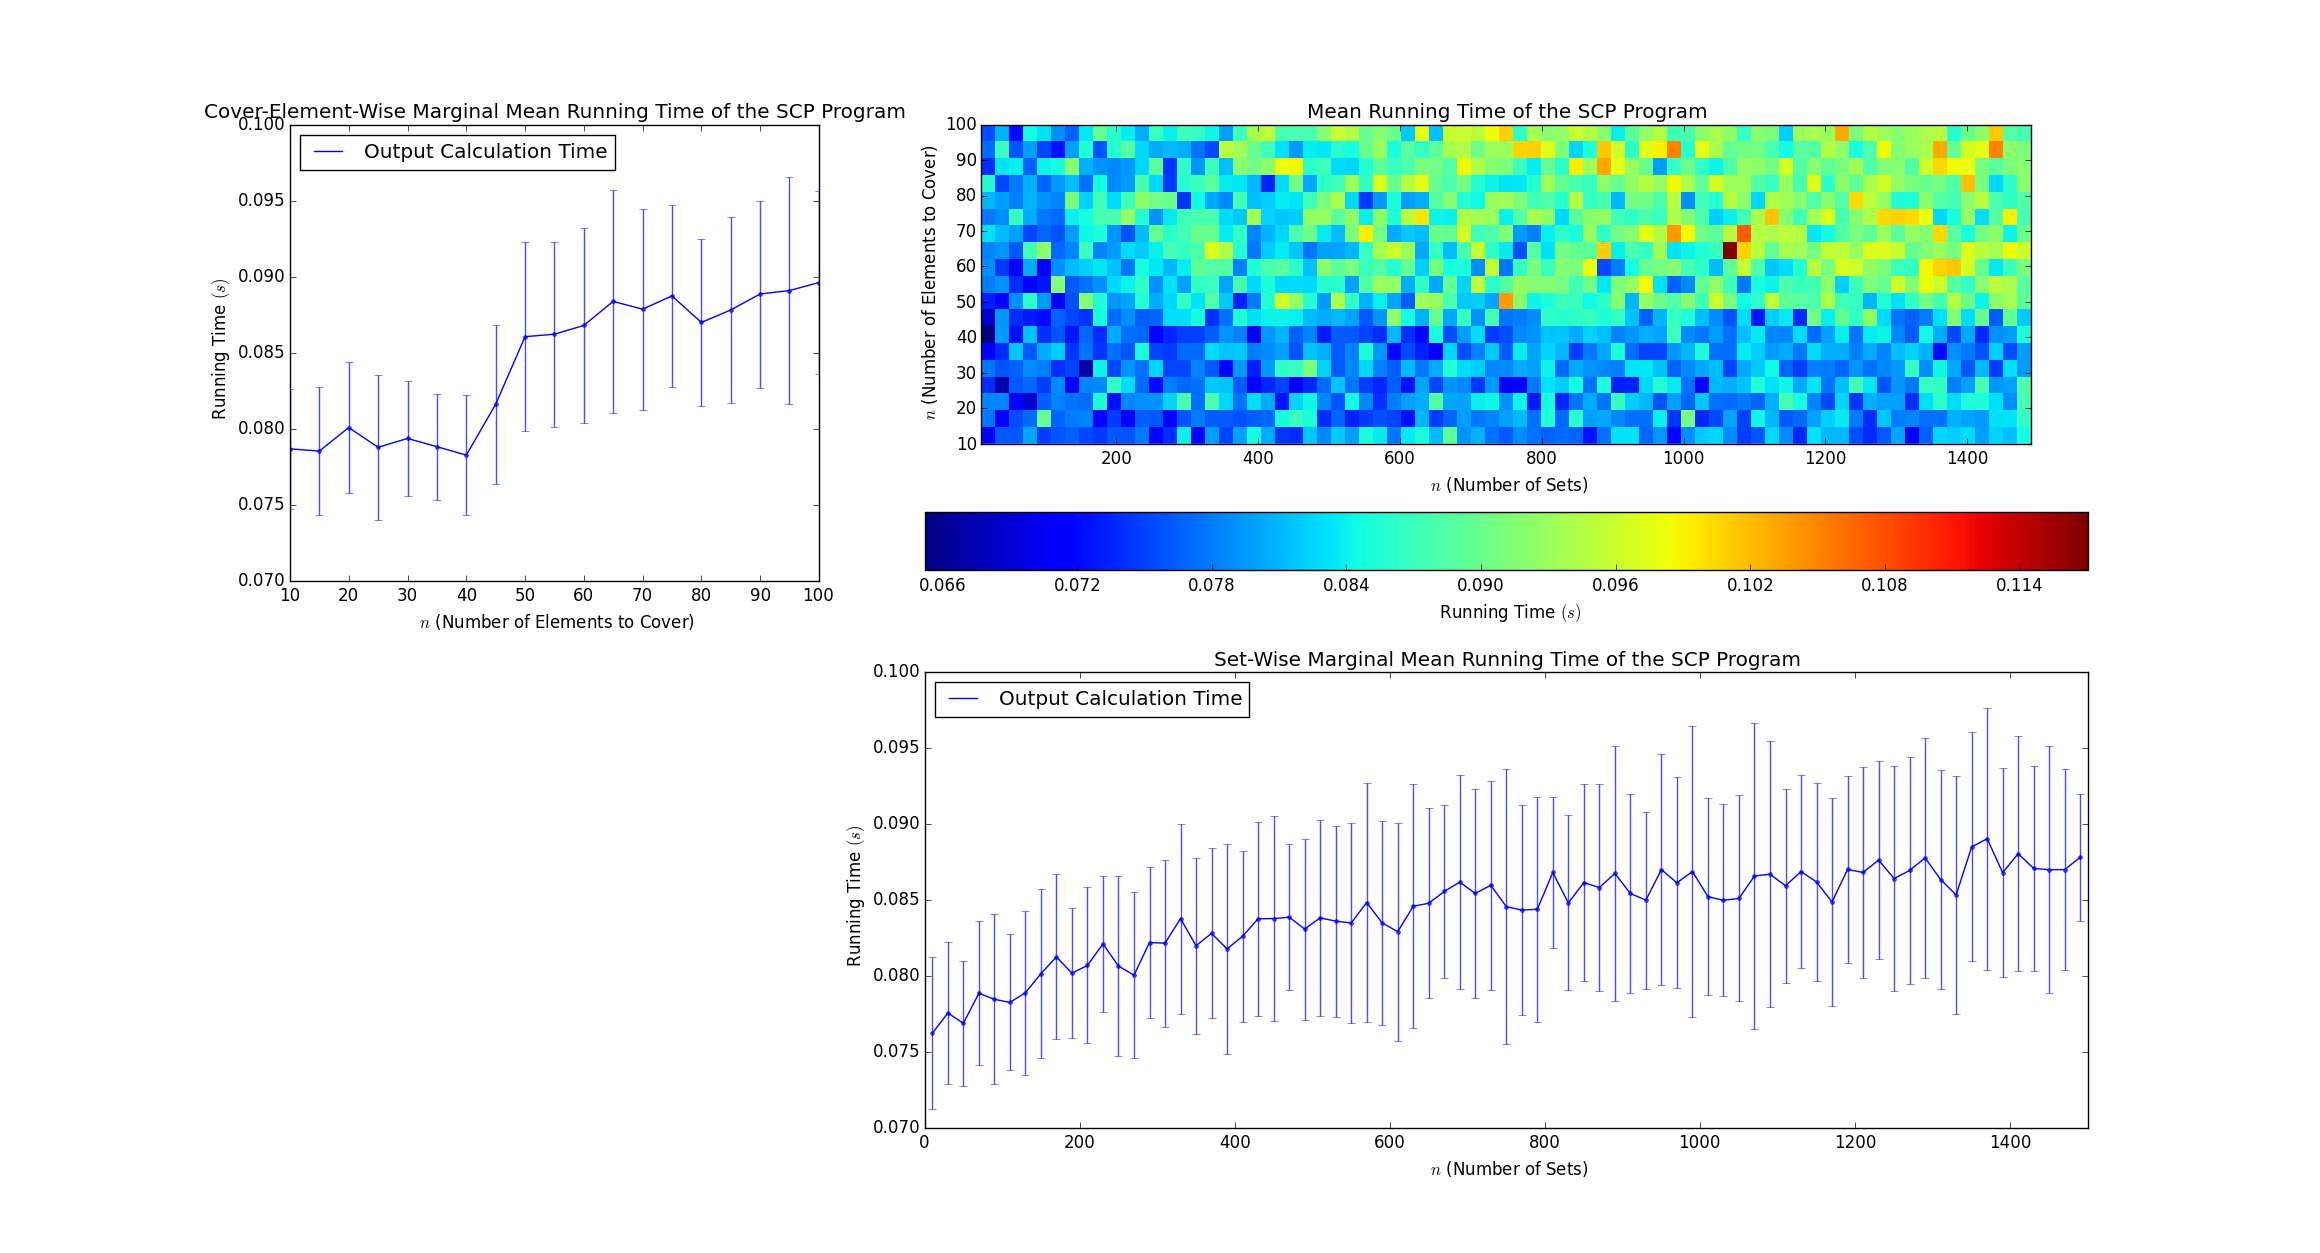
\includegraphics[width = 6.7in]{running_time_original_density0p3.png}}
	%  \vspace{2.0cm}
	\hfill
	
	%\vspace{-0.5cm}
	\caption{This figure displays the average running time performance of the ASP, over $20$ runs, for various instance configurations from the problem domain. All instances in this figure have a density of approximately $0.3$.}
	
	
\end{figure}


We construct an automated instance generation mechanism to provide randomly-constructed instances of the problem with some desired characteristics. This enables repeated runs to ensure statistically valid conclusions are drawn. In this work, all presented run times are the mean of $25$ independent runs. In order to explore the problem domain, we consider several combinations of number of set, number of cover-elements, and density, as is done in Section 4.5, Table 3.2 of \cite{graph_algorithms_cristofides}.


\begin{figure}[ht!] \label{fig:runtime_analysis_density0p6}
	
	
	
	\centering
	\centerline{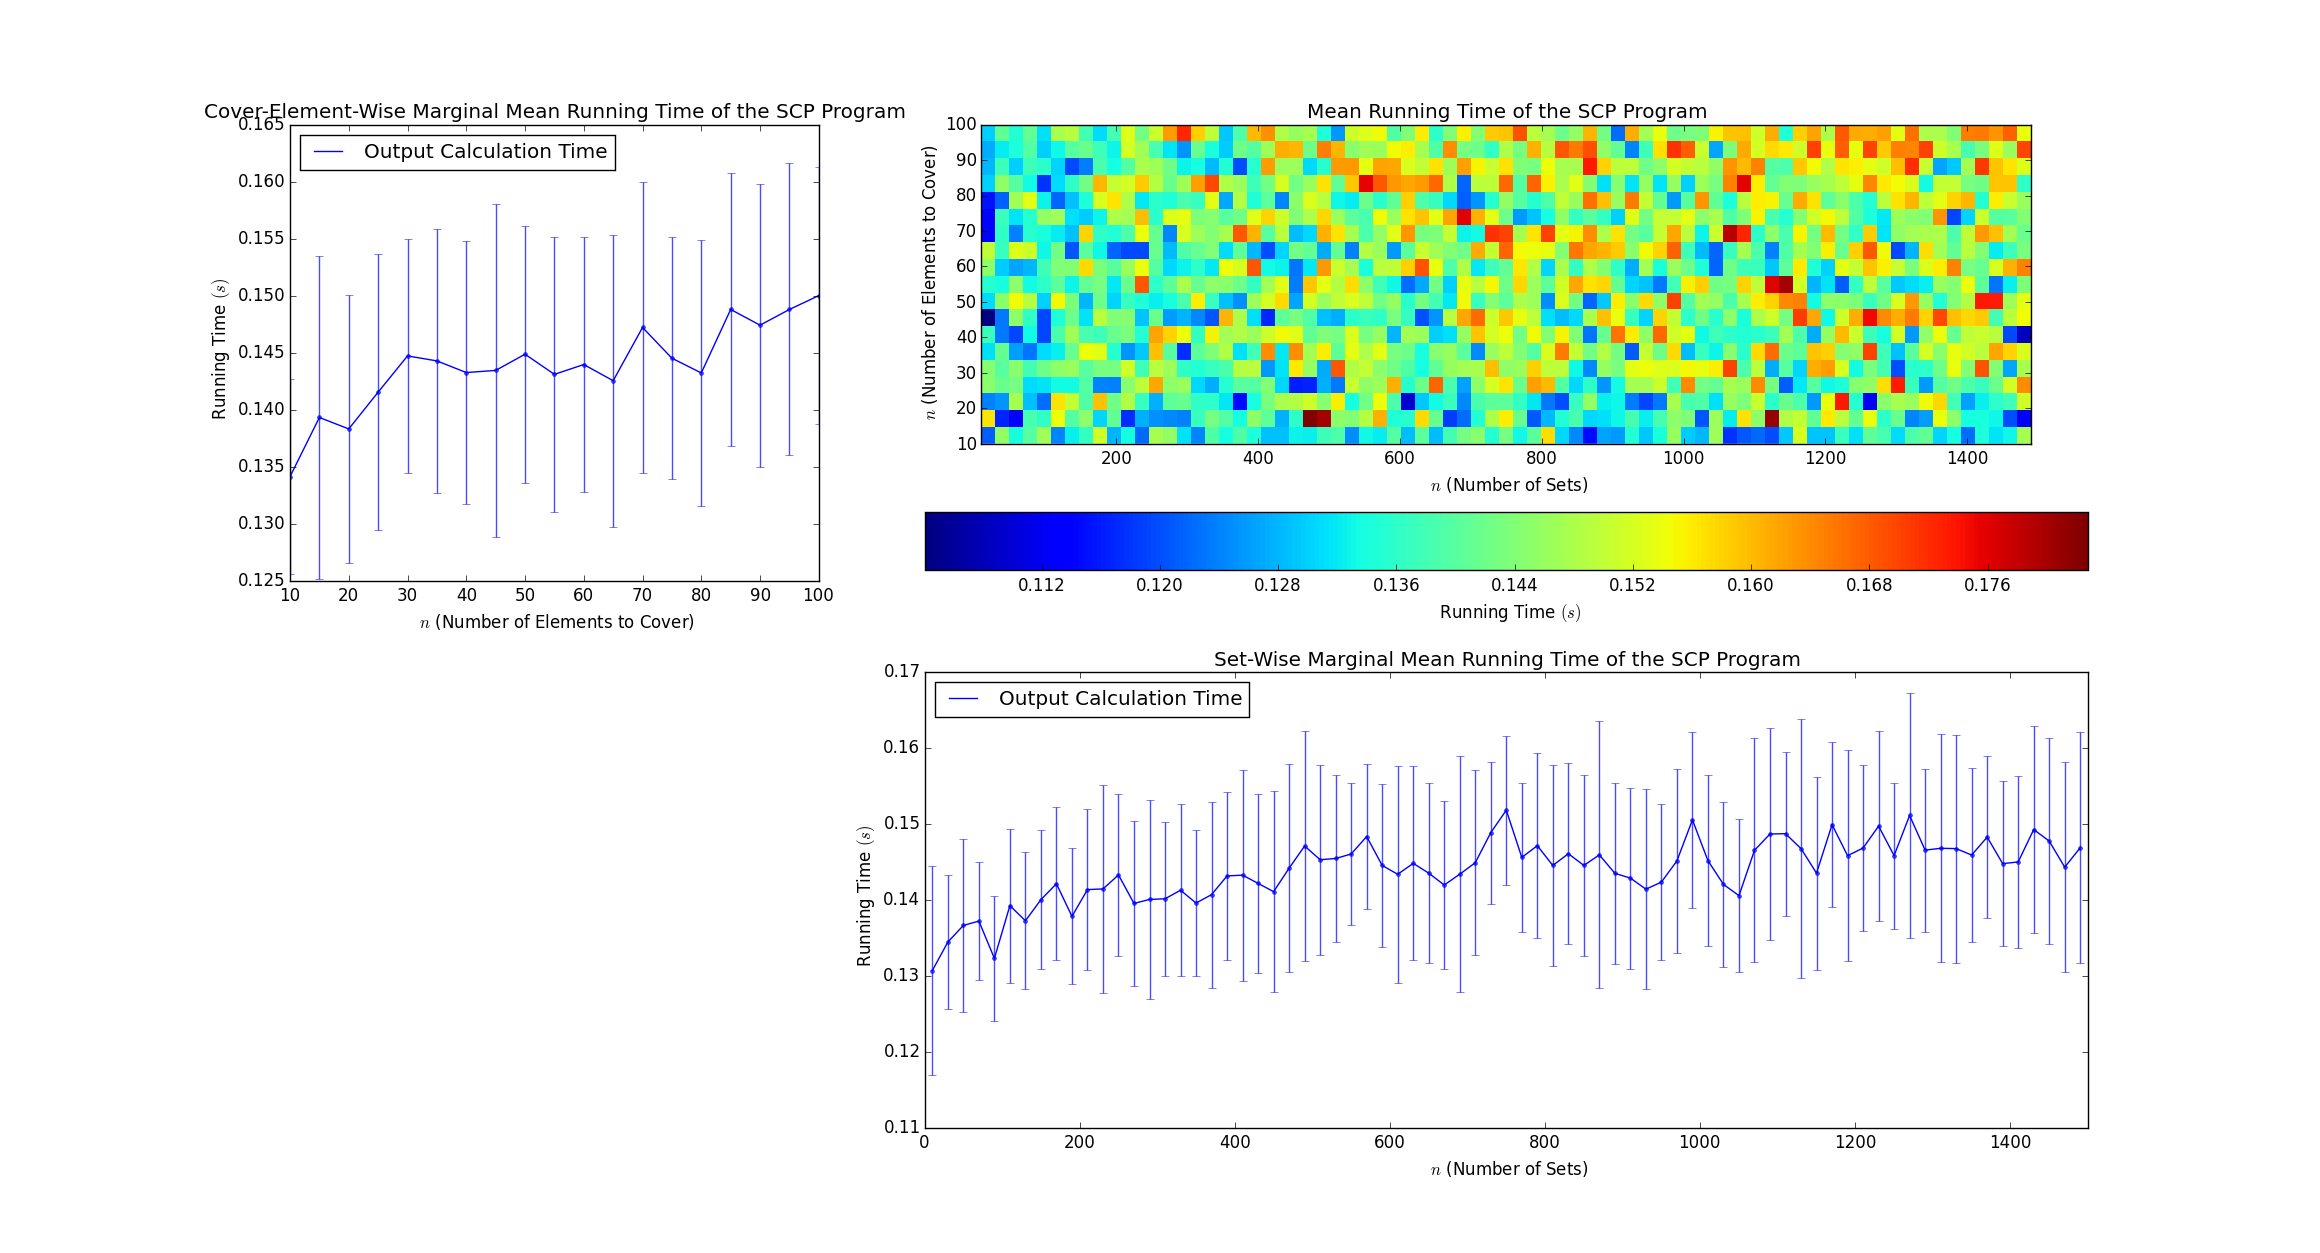
\includegraphics[width = 6.7in]{running_time_original_density0p6.png}}
	%  \vspace{2.0cm}
	\hfill
	
	%\vspace{-0.5cm}
	\caption{This figure displays the average running time performance of the ASP, over $20$ runs, for various instance configurations from the problem domain. All instances in this figure have a density of approximately $0.6$.}
	
	
\end{figure}

Figure~\ref{fig:runtime_analysis_density0p3} and Figure~\ref{fig:runtime_analysis_density0p6} display the results obtained by running the SCP solver. In each of these figures three plots are displayed, each of which highlights a particular element of the algorithms performance. The top-right plots are tile plots which show the mean running time, over $20$ runs, of the SCP program, for the number number of sets indicated on the horizontal axis, and the number os elements indicated on the vertical axis. The bottom-right plot displays the marginal mean and standard deviation of program running time, as the number of sets varies. These values are calculated by taking the mean and standard deviation of the mean running time values for a particular number of sets, across all numbers of elements to cover. The top-left plot shows the marginal mean and standard deviation of running time for a particular number of elements to cover across all numbers of sets.



Observing Figure~\ref{fig:runtime_analysis_density0p3}, we find several interesting trends. We find that the running time complexity of the ASP is approximately linear in both the number of cover elements and the number of covering sets. While this suggests that the ASP program runs in time of order $O(mn)$, where $m$ is the number of sets and $n$ is the number of elements to be covered, it does not necessarily prove it. It is possible that this trend does not hold in the asymptotic limit, given that the underlying problem is NP-complete. 
There is interesting non-linearity present in the small set-number limit, which is visible in the tile plot and the set-wise marginal plot for instances with number of sets less than $200$. In this limit, the number of elements to be covered has little effect on the running time of the algorithm. It is likely that increase in speed is due to early stopping, cause by the insufficiency of the covering sets to cover one or more of the cover elements.

In order to evaluate the sensitivity of the running time of the ASP to the density of the SCP instances, two identical experiments were conducted. The results of the first, in which all instances had a density of $0.3$ are show in Figure~\ref{fig:runtime_analysis_density0p3}. The results of the second, in which all instances had a density of $0.6,$ are shown in Figure~\ref{fig:runtime_analysis_density0p6}. Contrasting these two figures reveals an interesting relationship. First, not that there is a consistent and substantial higher-running-time bias in the higher-density case. Observe also that the mean running time behavior of the ASP, with respect to the number of sets in the instances, is biased but otherwise unchanged. Meanwhile, the running time behavior with respect to the number of elements is both biased \emph{and} has considerably higher variance. This implies that the running time of the ASP is more sensitive to the number of elements to be covered than the number of cover sets in the high-density limit. 

\subsection{ASP Limitations [c.3.3]} \label{scn:testing_limitations}

The limitations of the ASP were evaluated by producing sequentially more difficult SCP instances. We found that the ASP program was prohibitively long-running in experimental setups when the instance sizes grew beyond $100$ cover elements. Examining the performance of the program in isolated runs, we observe that instances with $150$ cover elements require approximately $35$ seconds. While for some problems, this may be acceptable, it is not acceptable for use in experiments consisting of many trials, which are have fixed delivery dates, such as the ones accomplished in support of this work

%\subsection{ASP Comparison [c.3.4]} \label{scn:testing_comparisons}

\pagebreak
\appendix		% Appendix begins here
	
\section{Code Listing}

\bibliographystyle{IEEEtran}
\bibliography{algorthimBib}

\end{document}
